\documentclass{beamer}
\usepackage{amsmath,graphics}
\usepackage{amssymb}

\usetheme{default}
\usepackage{xcolor}

\definecolor{solarizedBase03}{HTML}{002B36}
\definecolor{solarizedBase02}{HTML}{073642}
\definecolor{solarizedBase01}{HTML}{586e75}
\definecolor{solarizedBase00}{HTML}{657b83}
\definecolor{solarizedBase0}{HTML}{839496}
\definecolor{solarizedBase1}{HTML}{93a1a1}
\definecolor{solarizedBase2}{HTML}{EEE8D5}
\definecolor{solarizedBase3}{HTML}{FDF6E3}
\definecolor{solarizedYellow}{HTML}{B58900}
\definecolor{solarizedOrange}{HTML}{CB4B16}
\definecolor{solarizedRed}{HTML}{DC322F}
\definecolor{solarizedMagenta}{HTML}{D33682}
\definecolor{solarizedViolet}{HTML}{6C71C4}
%\definecolor{solarizedBlue}{HTML}{268BD2}
\definecolor{solarizedBlue}{HTML}{134676}
\definecolor{solarizedCyan}{HTML}{2AA198}
\definecolor{solarizedGreen}{HTML}{859900}
\definecolor{myBlue}{HTML}{162DB0}%{261CA4}
\setbeamercolor*{item}{fg=myBlue}
\setbeamercolor{normal text}{fg=solarizedBase03, bg=solarizedBase3}
\setbeamercolor{alerted text}{fg=myBlue}
\setbeamercolor{example text}{fg=myBlue, bg=solarizedBase3}
\setbeamercolor*{frametitle}{fg=solarizedRed}
\setbeamercolor*{title}{fg=solarizedRed}
\setbeamercolor{block title}{fg=myBlue, bg=solarizedBase3}
\setbeameroption{hide notes}
\setbeamertemplate{note page}[plain]
\beamertemplatenavigationsymbolsempty
\usefonttheme{professionalfonts}
\usefonttheme{serif}

\usepackage{fourier}

\def\vec#1{\mathchoice{\mbox{\boldmath$\displaystyle#1$}}
{\mbox{\boldmath$\textstyle#1$}}
{\mbox{\boldmath$\scriptstyle#1$}}
{\mbox{\boldmath$\scriptscriptstyle#1$}}}
\definecolor{OwnGrey}{rgb}{0.560,0.000,0.000} % #999999
\definecolor{OwnBlue}{rgb}{0.121,0.398,0.711} % #1f64b0
\definecolor{red4}{rgb}{0.5,0,0}
\definecolor{blue4}{rgb}{0,0,0.5}
\definecolor{Blue}{rgb}{0,0,0.66}
\definecolor{LightBlue}{rgb}{0.9,0.9,1}
\definecolor{Green}{rgb}{0,0.5,0}
\definecolor{LightGreen}{rgb}{0.9,1,0.9}
\definecolor{Red}{rgb}{0.9,0,0}
\definecolor{LightRed}{rgb}{1,0.9,0.9}
\definecolor{White}{gray}{1}
\definecolor{Black}{gray}{0}
\definecolor{LightGray}{gray}{0.8}
\definecolor{Orange}{rgb}{0.1,0.2,1}
\setbeamerfont{sidebar right}{size=\scriptsize}
\setbeamercolor{sidebar right}{fg=Black}

\renewcommand{\emph}[1]{{\textcolor{solarizedRed}{\itshape #1}}}

\newcommand\cA{\mathcal A}
\newcommand\cB{\mathcal B}
\newcommand\cC{\mathcal C}
\newcommand\cD{\mathcal D}
\newcommand\cE{\mathcal E}
\newcommand\cF{\mathcal F}
\newcommand\cG{\mathcal G}
\newcommand\cH{\mathcal H}
\newcommand\cI{\mathcal I}
\newcommand\cJ{\mathcal J}
\newcommand\cK{\mathcal K}
\newcommand\cL{\mathcal L}
\newcommand\cM{\mathcal M}
\newcommand\cN{\mathcal N}
\newcommand\cO{\mathcal O}
\newcommand\cP{\mathcal P}
\newcommand\cQ{\mathcal Q}
\newcommand\cR{\mathcal R}
\newcommand\cS{\mathcal S}
\newcommand\cT{\mathcal T}
\newcommand\cU{\mathcal U}
\newcommand\cV{\mathcal V}
\newcommand\cW{\mathcal W}
\newcommand\cX{\mathcal X}
\newcommand\cY{\mathcal Y}
\newcommand\cZ{\mathcal Z}

\newcommand\fA{\mathfrak A}
\newcommand\fB{\mathfrak B}
\newcommand\fC{\mathfrak C}
\newcommand\fD{\mathfrak D}
\newcommand\fE{\mathfrak E}
\newcommand\fF{\mathfrak F}
\newcommand\fG{\mathfrak G}
\newcommand\fH{\mathfrak H}
\newcommand\fI{\mathfrak I}
\newcommand\fJ{\mathfrak J}
\newcommand\fK{\mathfrak K}
\newcommand\fL{\mathfrak L}
\newcommand\fM{\mathfrak M}
\newcommand\fN{\mathfrak N}
\newcommand\fO{\mathfrak O}
\newcommand\fP{\mathfrak P}
\newcommand\fQ{\mathfrak Q}
\newcommand\fR{\mathfrak R}
\newcommand\fS{\mathfrak S}
\newcommand\fT{\mathfrak T}
\newcommand\fU{\mathfrak U}
\newcommand\fV{\mathfrak V}
\newcommand\fW{\mathfrak W}
\newcommand\fX{\mathfrak X}
\newcommand\fY{\mathfrak Y}
\newcommand\fZ{\mathfrak Z}

\newcommand\fa{\mathfrak a}
\newcommand\fb{\mathfrak b}
\newcommand\fc{\mathfrak c}
\newcommand\fd{\mathfrak d}
\newcommand\fe{\mathfrak e}
\newcommand\ff{\mathfrak f}
\newcommand\fg{\mathfrak g}
\newcommand\fh{\mathfrak h}
%\newcommand\fi{\mathfrak i}
\newcommand\fj{\mathfrak j}
\newcommand\fk{\mathfrak k}
\newcommand\fl{\mathfrak l}
\newcommand\fm{\mathfrak m}
\newcommand\fn{\mathfrak n}
\newcommand\fo{\mathfrak o}
\newcommand\fp{\mathfrak p}
\newcommand\fq{\mathfrak q}
\newcommand\fr{\mathfrak r}
\newcommand\fs{\mathfrak s}
\newcommand\ft{\mathfrak t}
\newcommand\fu{\mathfrak u}
\newcommand\fv{\mathfrak v}
\newcommand\fw{\mathfrak w}
\newcommand\fx{\mathfrak x}
\newcommand\fy{\mathfrak y}
\newcommand\fz{\mathfrak z}

\newcommand\vA{\vec A}
\newcommand\vB{\vec B}
\newcommand\vC{\vec C}
\newcommand\vD{\vec D}
\newcommand\vE{\vec E}
\newcommand\vF{\vec F}
\newcommand\vG{\vec G}
\newcommand\vH{\vec H}
\newcommand\vI{\vec I}
\newcommand\vJ{\vec J}
\newcommand\vK{\vec K}
\newcommand\vL{\vec L}
\newcommand\vM{\vec M}
\newcommand\vN{\vec N}
\newcommand\vO{\vec O}
\newcommand\vP{\vec P}
\newcommand\vQ{\vec Q}
\newcommand\vR{\vec R}
\newcommand\vS{\vec S}
\newcommand\vT{\vec T}
\newcommand\vU{\vec U}
\newcommand\vV{\vec V}
\newcommand\vW{\vec W}
\newcommand\vX{\vec X}
\newcommand\vY{\vec Y}
\newcommand\vZ{\vec Z}

\newcommand\va{\vec a}
\newcommand\vb{\vec b}
\newcommand\vc{\vec c}
\newcommand\vd{\vec d}
\newcommand\ve{\vec e}
\newcommand\vf{\vec f}
\newcommand\vg{\vec g}
\newcommand\vh{\vec h}
\newcommand\vi{\vec i}
\newcommand\vj{\vec j}
\newcommand\vk{\vec k}
\newcommand\vl{\vec l}
\newcommand\vm{\vec m}
\newcommand\vn{\vec n}
\newcommand\vo{\vec o}
\newcommand\vp{\vec p}
\newcommand\vq{\vec q}
\newcommand\vr{\vec r}
\newcommand\vs{\vec s}
\newcommand\vt{\vec t}
\newcommand\vu{\vec u}
\newcommand\vv{\vec v}
\newcommand\vw{\vec w}
\newcommand\vx{\vec x}
\newcommand\vy{\vec y}
\newcommand\vz{\vec z}

\renewcommand\AA{\mathbb A}
\newcommand\NN{\mathbb N}
\newcommand\ZZ{\mathbb Z}
\newcommand\PP{\mathbb P}
\newcommand\QQ{\mathbb Q}
\newcommand\RR{\mathbb R}
\renewcommand\SS{\mathbb S}
\newcommand\CC{\mathbb C}

\newcommand{\id}{\mathrm{id}}
\newcommand{\pr}{\mathrm{P}}
\newcommand{\Vol}{\mathrm{vol}}
\newcommand\norm[1]{\left\|{#1}\right\|} 
\newcommand\sign{\mathrm{sign}}
\newcommand{\eps}{\varepsilon}
\newcommand{\abs}[1]{\left|#1\right|}
\newcommand\bc[1]{\left({#1}\right)} 
\newcommand\cbc[1]{\left\{{#1}\right\}} 
\newcommand\bcfr[2]{\bc{\frac{#1}{#2}}} 
\newcommand{\bck}[1]{\left\langle{#1}\right\rangle} 
\newcommand\brk[1]{\left\lbrack{#1}\right\rbrack} 
\newcommand\scal[2]{\bck{{#1},{#2}}} 
\newcommand{\vecone}{\mathbb{1}}
\newcommand{\tensor}{\otimes}
\newcommand{\diag}{\mathrm{diag}}
\newcommand{\ggt}{\mathrm{ggT}}
\newcommand{\kgv}{\mathrm{kgV}}

\newcommand{\Karonski}{Karo\'nski}
\newcommand{\Erdos}{Erd\H{o}s}
\newcommand{\Renyi}{R\'enyi}
\newcommand{\Lovasz}{Lov\'asz}
\newcommand{\Juhasz}{Juh\'asz}
\newcommand{\Bollobas}{Bollob\'as}
\newcommand{\Furedi}{F\"uredi}
\newcommand{\Komlos}{Koml\'os}
\newcommand{\Luczak}{\L uczak}
\newcommand{\Kucera}{Ku\v{c}era}
\newcommand{\Szemeredi}{Szemer\'edi}

\renewcommand{\ae}{\"a}
\renewcommand{\oe}{\"o}
\newcommand{\ue}{\"u}
\newcommand{\Ae}{\"A}
\newcommand{\Oe}{\"O}
\newcommand{\Ue}{\"U}

\title[Linadi]{Die symmetrische Gruppe}
\author[Amin Coja-Oghlan]{Amin Coja-Oghlan}
\institute[Frankfurt]{JWGUFFM}
\date{}

\begin{document}

\frame[plain]{\titlepage}

\begin{frame}\frametitle{Die symmetrische Gruppe}
\begin{block}{Erinnerung}
\begin{itemize}
\item Die symmetrische Gruppe $\SS_n$ besteht aus allen bijektiven Abbildungen
	\begin{align*}
		\{1,\ldots,n\}\to\{1,\ldots,n\}
	\end{align*}
\item Diese Abbildungen werden auch \emph{Permutationen} genannt.
\end{itemize}
\end{block}
\end{frame}

\begin{frame}\frametitle{Die symmetrische Gruppe}
	\begin{block}{Proposition}
		F\ue r jedes $n\in\NN$ gilt $|\SS_n|=n!$\enspace.
	\end{block}
%	\begin{overprint}
%		\onslide<1>	
%		\begin{block}{Beweis}
%			\begin{itemize}
%				\item Induktion nach $n$.	
%				\item F\ue r $n=1$ gilt $|\SS_n|=1=n!\enspace$.
%				\item Zum Schlu\ss\ von $n$ auf $n+1$ sei $\sigma\in\SS_{n+1}$.
%				\item Dann gibt es $x,y\in\{1,\ldots,n+1\}$ mit
%					\begin{align*}
%						\sigma(n+1)&=x,&\sigma(y)=n+1.
%					\end{align*}
%				\item ($x,y$ k\oe nnen gleich sein und auch $x=y=n+1$ ist m\oe glich.)
%			\end{itemize}
%		\end{block}
%		\onslide<2>
%		\begin{block}{Beweis (Fortsetzung)}
%			\begin{itemize}
%				\item Definiere $\sigma':\{1,\ldots,n\}\to\{1,\ldots,n\}$ durch
%					\begin{align*}
%						\sigma'(y)&=x,&&\sigma'(z)=\sigma(z)\mbox{ f\ue r alle }z\neq y.
%					\end{align*}
%				\item Dann ist $\sigma'\in\SS_n$.
%				\item Au\ss erdem kann man $\sigma$ aus $\sigma'$ und $x$ rekonstruieren.
%				\item Also gilt $|\SS_{n+1}|\leq |\SS_n|\cdot(n+1)=n!\cdot(n+1)=(n+1)!$.
%			\end{itemize}
%		\end{block}
%		\onslide<3>
%		\begin{block}{Beweis (Fortsetzung)}
%			\begin{itemize}
%				\item Ist umgekehrt $\tau'\in\SS_n$ und $x\in\{1,\ldots,n+1\}$, so definieren wir $\tau:\{1,\ldots,n+1\}\to\{1,\ldots,n+1\}$ durch
%					\begin{align*}
%						\tau(n+1)&=x\\
%						\tau(y)&=n+1\qquad\mbox{falls }\tau'(y)=x,\\
%						\tau(z)&=\tau'(z)\qquad\mbox{falls }\tau'(z)\neq x.
%					\end{align*}
%				\item Es gilt $\tau\in\SS_{n+1}$ und $(\tau',x)$ kann aus $\tau$ rekonstruiert werden.
%				\item Daraus folgt $|\SS_{n+1}|\geq|\SS_n|\cdot(n+1)=n!\cdot(n+1)=(n+1)!.$
%			\end{itemize}
%		\end{block}
%	\end{overprint}
\end{frame}

\begin{frame}\frametitle{Die symmetrische Gruppe}
	\begin{block}{Beispiel}
		F\ue r $n=3$ erhalten wir die symmetrische Gruppe $\SS_3$ mit $3!=3\cdot2\cdot1=6$ Elementen:
		\begin{align*}
			\sigma_1:1&\mapsto 1,&2\mapsto&2,&3\mapsto3\\
			\sigma_2:1&\mapsto 1,&2\mapsto&3,&3\mapsto2\\
			\sigma_3:1&\mapsto 2,&2\mapsto&1,&3\mapsto3\\
			\sigma_4:1&\mapsto 2,&2\mapsto&3,&3\mapsto1\\
			\sigma_5:1&\mapsto 3,&2\mapsto&2,&3\mapsto1\\
			\sigma_6:1&\mapsto 3,&2\mapsto&1,&3\mapsto2
		\end{align*}
	\end{block}
\end{frame}

\begin{frame}\frametitle{Die symmetrische Gruppe}
	\begin{block}{Definition}
		Eine Permutation $\theta\in\SS_n$ hei\ss t eine \emph{Transposition}, falls es Zahlen $1\leq x<y\leq n$ gibt mit
		\begin{align*}
			\theta(x)&=y,&\theta(y)&=x,&\theta(z)=z&&\mbox{ f\ue r alle }z\in\{1,\ldots,n\}\setminus\{x,y\}.
		\end{align*}
	\end{block}
\end{frame}

\begin{frame}\frametitle{Die symmetrische Gruppe}
	\hfill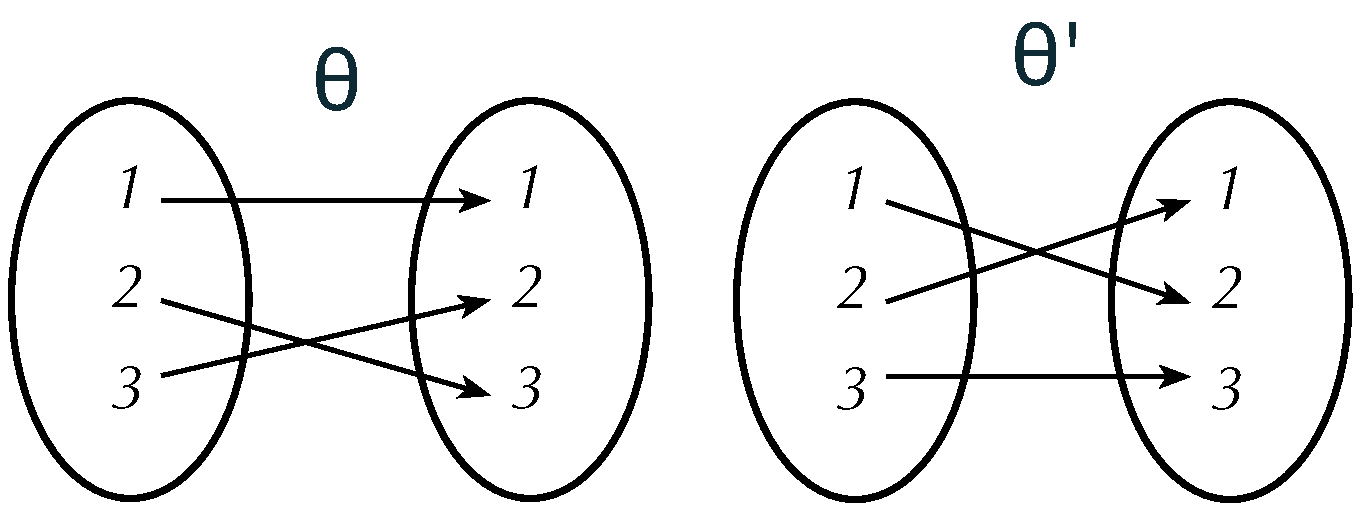
\includegraphics[height=20mm]{pics/transpositions3.pdf}
	\begin{block}{Beispiel}
		\begin{itemize}
			\item f\ue r $n=3$ sind
				\begin{align*}
					\theta:1&\mapsto1&2&\mapsto3&3&\mapsto2\\
					\theta':1&\mapsto2&2&\mapsto1&3&\mapsto3
				\end{align*}
				Transpositionen.
		\end{itemize}
	\end{block}
\end{frame}

\begin{frame}\frametitle{Die symmetrische Gruppe}
	\hfill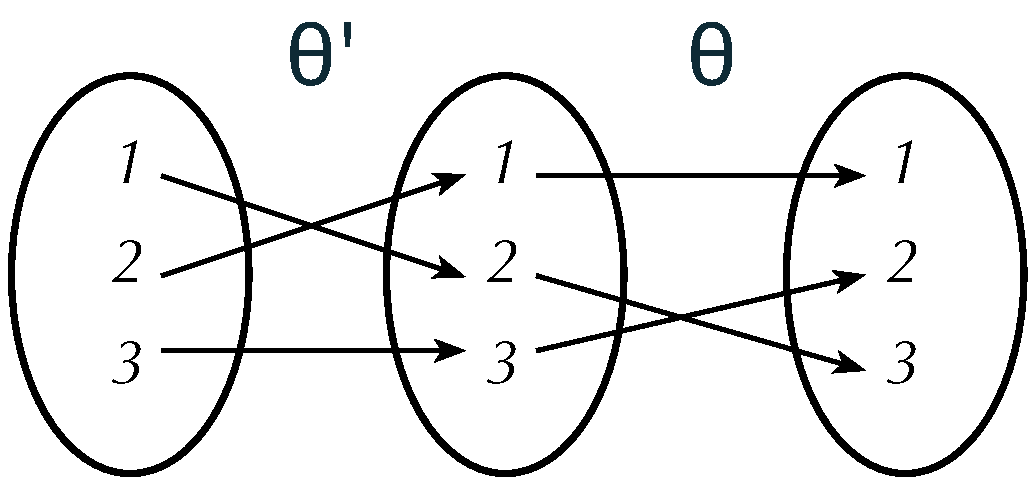
\includegraphics[height=20mm]{pics/transpositions.pdf}\hfill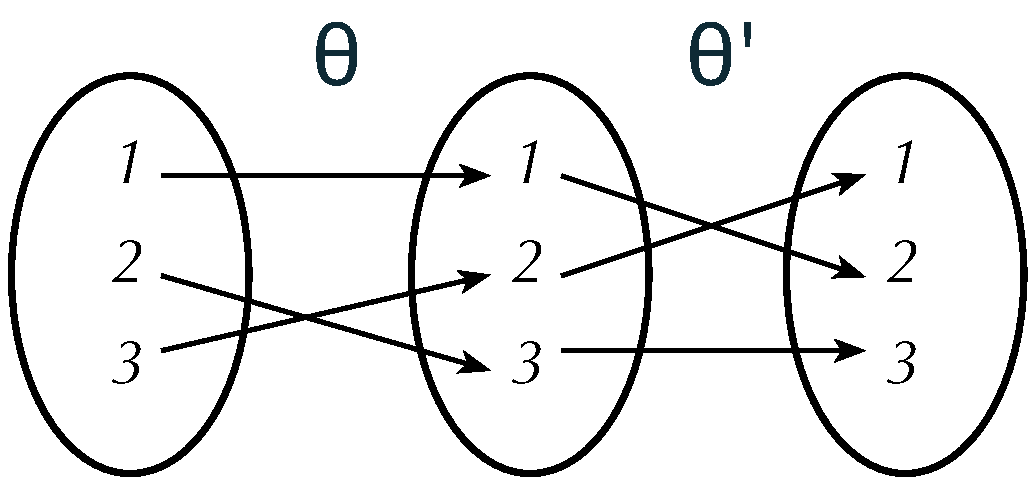
\includegraphics[height=20mm]{pics/transpositions2.pdf}
	\begin{block}{Beispiel}
		\begin{itemize}
			\item die Transpositionen $\theta,\theta'$ kommutieren nicht:
				\begin{align*}
					\theta\circ\theta':1&\mapsto3&2&\mapsto1&3\mapsto2\\
					\theta'\circ\theta:1&\mapsto2&2&\mapsto3&3\mapsto1
				\end{align*}
			\item es gilt also $\theta'\circ\theta\neq\theta\circ\theta'$
		\end{itemize}
	\end{block}
\end{frame}

\begin{frame}\frametitle{Die symmetrische Gruppe}
	\begin{block}{Proposition}
		Zu jeder Permutation $\sigma\in\SS_n$ gibt eine Zahl $\ell\geq1$ und Transpositionen $\theta_1,\ldots,\theta_\ell$, so da\ss\ $$ \sigma=\theta_1\circ\theta_2\circ\cdots\circ\theta_\ell.  $$
	\end{block}
%	\begin{overprint}
%		\onslide<1>
%		\begin{block}{Beweis}
%			\begin{itemize}
%				\item Induktion nach $n$; f\ue r $n=1$ ist nichts zu zeigen.
%				\item Zum Schlu\ss\ auf $n+1$ sei $\sigma\in\SS_{n+1}$.
%				\item Finde $x,y$ mit $\sigma(n+1)=x$ und $\sigma(y)=n+1$.
%				\item Dann ist $\sigma':\{1,\ldots,n+1\}\to\{1,\ldots,n+1\}$ mit
%					\begin{align*}
%						\sigma'(y)&=x,&\sigma'(n+1)&=n+1,&\sigma'(z)&=\sigma(z)\mbox{ f\ue r }z\neq y,n+1
%					\end{align*}
%					eine Permutation.
%			\end{itemize}	
%		\end{block}
%		\onslide<2>
%		\begin{block}{Beweis}
%			\begin{itemize}
%				\item Nach Induktion gibt es Transpositionen $\theta_1,\ldots,\theta_\ell$ von $1,\ldots,n$, so da\ss\
%					\begin{align*}
%						\sigma'=\theta_1\circ\cdots\circ\theta_\ell.
%					\end{align*}
%				\item Sei nun $\theta_0$ die Transposition
%					\begin{align*}
%						\theta_0(x)&=n+1,&\theta_0(n+1)&=x.
%					\end{align*}
%				\item Dann gilt $\sigma=\theta_0\circ\sigma'=\theta_0\circ\theta_1\circ\cdots\circ\theta_\ell$.
%			\end{itemize}	
%		\end{block}
%	\end{overprint}
\end{frame}

\begin{frame}\frametitle{Die symmetrische Gruppe}
	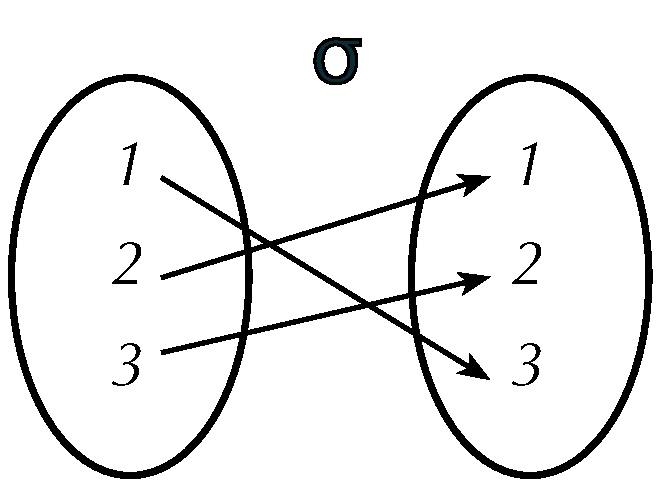
\includegraphics[height=20mm]{pics/sigma.pdf}\hfill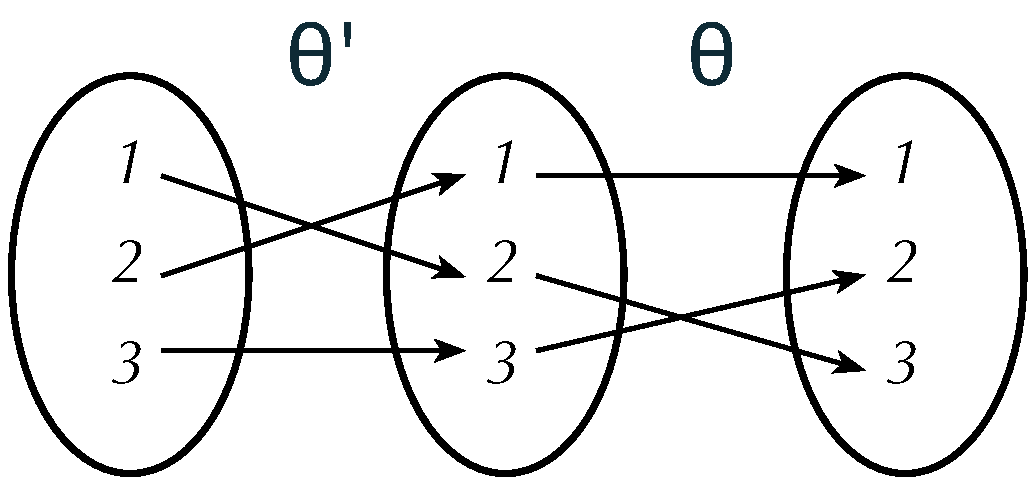
\includegraphics[height=20mm]{pics/transpositions.pdf}
	\begin{block}{Beispiel}
		\begin{itemize}
			\item Betrachte die folgende Permutation $\sigma\in\SS_3$:
				\begin{align*}
					\sigma:1&\mapsto 3,&2&\mapsto 1,&3&\mapsto 2.
				\end{align*}
			\item Seien $\theta,\theta'$ die Transpositionen 
				\begin{align*}
					\theta:1&\mapsto 1,&2&\mapsto 3,&3\mapsto 2,\\
					\theta':1&\mapsto 2,&1&\mapsto 2,&3\mapsto 3.
				\end{align*}
			\item Dann gilt $\sigma=\theta\circ\theta'.$
		\end{itemize}
	\end{block}
\end{frame}

\begin{frame}\frametitle{Die symmetrische Gruppe}
	\begin{block}{Definition}
		Zu $\sigma\in\SS_n$ hei\ss t
		\begin{align*}
			\sign(\sigma)&=\prod_{1\leq i<j\leq n}\frac{\sigma(i)-\sigma(j)}{i-j}
		\end{align*}
		das \emph{Vorzeichen} oder \emph{Signum} der Permutation $\sigma$.
	\end{block}
\end{frame}

\begin{frame}\frametitle{Die symmetrische Gruppe}
	\begin{block}{Beispiel}
		\begin{itemize}
			\item Betrachte die folgende Permutation $\sigma\in\SS_3$:
				\begin{align*}
					\sigma:1&\mapsto 3,&2&\mapsto 1,&3&\mapsto 2.
				\end{align*}
			\item Dann erhalten wir
				\begin{align*}
					\sign(\sigma)&=\frac{\sigma(1)-\sigma(2)}{1-2}\cdot\frac{\sigma(1)-\sigma(3)}{1-3}\cdot\frac{\sigma(2)-\sigma(3)}{2-3}\\
								 &=\frac{3-1}{1-2}\cdot\frac{3-2}{1-3}\cdot\frac{1-2}{2-3}\\&=1.
				\end{align*}
		\end{itemize}
	\end{block}
\end{frame}

\begin{frame}\frametitle{Die symmetrische Gruppe}
	\begin{block}{Beispiel}
		\begin{itemize}
			\item Betrachte die folgende Transposition $\theta\in\SS_3$:
				\begin{align*}
					\theta:&1\mapsto 2,&2&\mapsto 1,&3&\mapsto 3.
				\end{align*}
			\item Dann erhalten wir
				\begin{align*}
					\sign(\sigma)&=\frac{\sigma(1)-\sigma(2)}{1-2}\cdot\frac{\sigma(1)-\sigma(3)}{1-3}\cdot\frac{\sigma(2)-\sigma(3)}{2-3}\\
								 &=\frac{2-1}{1-2}\cdot\frac{2-3}{1-3}\cdot\frac{1-3}{2-3}\\&=-1.
				\end{align*}
			\item Allgemeiner gilt f\ue r \emph{jede} Transposition $\theta\in\SS_n$:
				\begin{align*}
					\sign(\theta)&=-1.
				\end{align*}
		\end{itemize}
	\end{block}
\end{frame}

\begin{frame}\frametitle{Die symmetrische Gruppe}
	\begin{block}{Proposition}
		F\ue r alle $\sigma,\tau\in\SS_n$ gilt	$\sign(\sigma\circ\tau)=\sign(\sigma)\cdot\sign(\tau).$
	\end{block}
	\begin{block}{Beweis}
		\begin{align*}
			\sign(\sigma\circ\tau)&=\prod_{i<j}\frac{\sigma(\tau(i))-\sigma(\tau(j))}{i-j}\\
								  &=\prod_{i<j}\frac{\sigma(\tau(i))-\sigma(\tau(j))}{\tau(i)-\tau(j)}\cdot\frac{\tau(i)-\tau(j)}{i-j}\\
								  &=\prod_{i<j}\frac{\sigma(\tau(i))-\sigma(\tau(j))}{\tau(i)-\tau(j)}\cdot\prod_{i<j}\frac{\tau(i)-\tau(j)}{i-j}\\
								  &=\prod_{i<j}\frac{\sigma(i)-\sigma(j)}{i-j}\cdot\prod_{i<j}\frac{\tau(i)-\tau(j)}{i-j}\\
								  &=\sign(\sigma)\cdot\sign(\tau).
		\end{align*}	
	\end{block}
\end{frame}

\begin{frame}\frametitle{Die symmetrische Gruppe}
	\begin{block}{Korollar}
		F\ue r alle $\sigma\in\SS_n$ gilt	$\sign(\sigma)\in\{1,-1\}$.
	\end{block}
	\begin{overprint}
		\onslide<1>
		\begin{block}{Beweis}
			\begin{itemize}
				\item Jede Permutation $\sigma$ kann als Produkt von Transposition geschrieben werden:
					\begin{align*}
						\sigma&=\theta_1\circ\cdots\circ\theta_\ell.
					\end{align*}
				\item F\ue r jede Transposition gilt $\sign(\theta_i)=-1$.
				\item Die Proposition zeigt also:
					\begin{align*}
						\sign(\sigma)&=\prod_{i=1}^\ell\sign(\theta_i)=(-1)^\ell\in\{-1,1\}.
					\end{align*}
			\end{itemize}	
		\end{block}	
		\onslide<2>
		\begin{block}{Anmerkung}
			\begin{itemize}
				\item Es gilt $\sign(\sigma)=1$, wenn $\sigma$ sich als Produkt einer \emph{geraden} Zahl von Transpositionen schreiben l\ae\ss t.
				\item Sonst gilt $\sign(\sigma)=-1$.
				\item $\sign$ ein Homomorphismus von $(\SS_n,\circ)$ auf $(\{-1,1\},\,\cdot\,)$.
				\item Die Menge
					\begin{align*}
						\AA_n&=\cbc{\sigma\in\SS_n:\sign(\sigma)=1}
					\end{align*}
					ist mit der Verkn\ue pfung $\circ$ selbst eine Gruppe.
				\item Sie hei\ss t die \emph{Alternierende Gruppe}.
			\end{itemize}
		\end{block}
	\end{overprint}
\end{frame}

\begin{frame}\frametitle{Die symmetrische Gruppe}
\begin{block}{Definition}
	Eine Permutation $\sigma\in\SS_n$ hei\ss t ein \emph{Zykel}, falls es verschiedene Zahlen $$i_1,i_2,\ldots,i_k\in\{1,\ldots,n\}$$ gibt, so da\ss
	\begin{align*}
		\sigma(i_j)&=i_{j+1}&&\mbox{f\ue r }1\leq j<k,\\
		\sigma(i_k)&=i_1.
	\end{align*}
	Wir nennen $k$ die \emph{L\ae nge} des Zykels.
\end{block}
\begin{block}{Anmerkung}
	Es gilt $k=\mathrm{ord}_{\SS_n}\sigma$.
\end{block}
\end{frame}

\begin{frame}\frametitle{Die symmetrische Gruppe}
	\hfill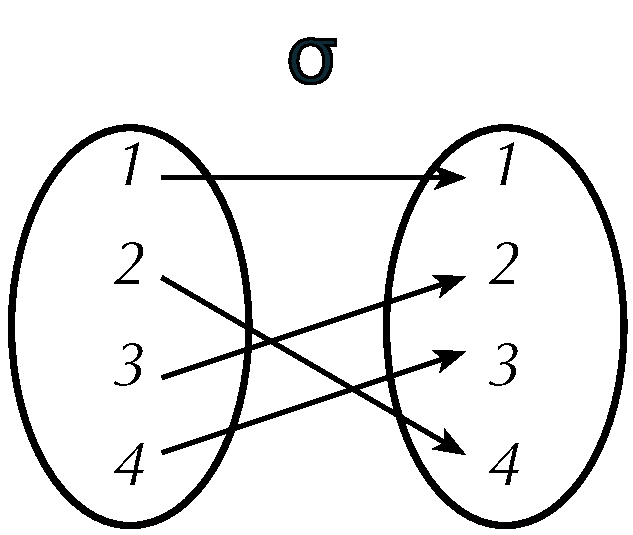
\includegraphics[height=25mm]{pics/cycle.pdf}
	\begin{block}{Beispiel}
		\begin{itemize}
			\item f\ue r $n=4$ ist die Permutation 
				\begin{align*}
					\sigma:1&\mapsto1&2&\mapsto4&3&\mapsto2&4&\mapsto3
				\end{align*}
				ein Zykel.
			\item Die L\ae nge des Zykels ist $k=3$ und
				\begin{align*}
					i_1&=2&i_2&=4&i_3&=3.
				\end{align*}
			\item Jede Transposition ist ein Zykel der L\ae nge $2$.
		\end{itemize}
	\end{block}
\end{frame}

\begin{frame}\frametitle{Die symmetrische Gruppe}
	\begin{block}{Zykelschreibweise}
		Sei $n\in\NN$ und seien $i_1,i_2,\ldots,i_k\in\{1,\ldots,n\}$ paarweise verschieden.
		Dann bezeichnet
		\begin{align*}
			(i_1\ i_2\ \cdots i_k)
		\end{align*}
		die Permutation
		\begin{align*}
			i_1&\mapsto i_2\\i_2&\mapsto i_3\\\vdots\\ i_{k-1}&\mapsto i_k\\i_k&\mapsto i_1\\
			j&\mapsto j\qquad\mbox{f\ue r alle }j\not\in\{i_1,\ldots,i_k\}.
		\end{align*}
	\end{block}
\end{frame}

\begin{frame}\frametitle{Die symmetrische Gruppe}
	\hfill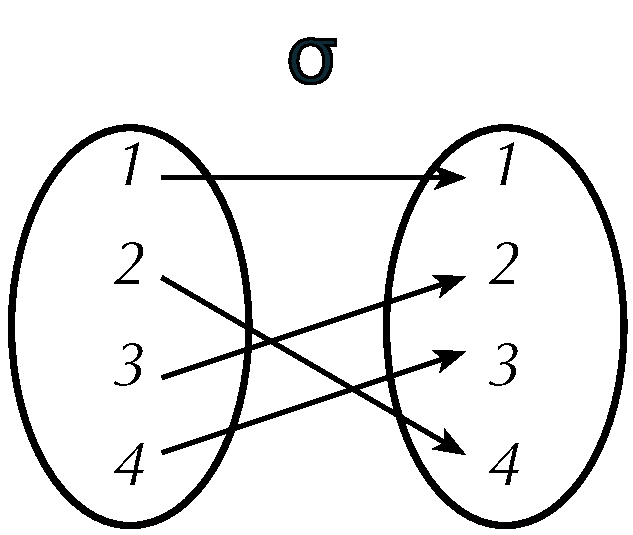
\includegraphics[height=25mm]{pics/cycle.pdf}
	\begin{block}{Beispiel}
		\begin{itemize}
			\item f\ue r $n=4$ betrachte die Permutation 
				\begin{align*}
					\sigma:1&\mapsto1&2&\mapsto4&3&\mapsto2&4&\mapsto3
				\end{align*}
				aus dem letzten Beispiel.
			\item Wir k\oe nnen $\sigma$  in Zykelschreibweise darstellen:
				\begin{align*}
					\sigma&=(2\quad4\quad3).
				\end{align*}
		\end{itemize}
	\end{block}
\end{frame}

\begin{frame}\frametitle{Die symmetrische Gruppe}
	\begin{block}{Definition}
		Zwei Zykel
		\begin{align*}
			\bc{i_1\ i_2\ \cdots\ i_k}\qquad\mbox{und}\qquad\bc{j_1\ j_2\ \cdots\ j_\ell}
		\end{align*}
		sind \emph{disjunkt}, wenn
		\begin{align*}
			\cbc{i_1,i_2,\ldots,i_k}\cap\cbc{j_1,j_2,\ldots,j_k}&=\emptyset.
		\end{align*}
	\end{block}
\end{frame}

\begin{frame}\frametitle{Die symmetrische Gruppe}
	\begin{block}{Satz}
		Zu jeder Zahl $n\in\NN$ und jeder Permutation $\sigma\in\SS_n$ existieren disjunkte Zykel $\zeta_1,\zeta_2,\ldots,\zeta_\ell$, so da\ss
		\begin{align*}
			\sigma&=\zeta_1\circ\zeta_2\circ\cdots\circ\zeta_\ell.
		\end{align*}
	\end{block}
	\begin{block}{Anmerkung}
		Bis auf die Reihenfolge sind die Zykel eindeutig bestimmt.
	\end{block}
\end{frame}

\begin{frame}\frametitle{Die symmetrische Gruppe}
	\hfill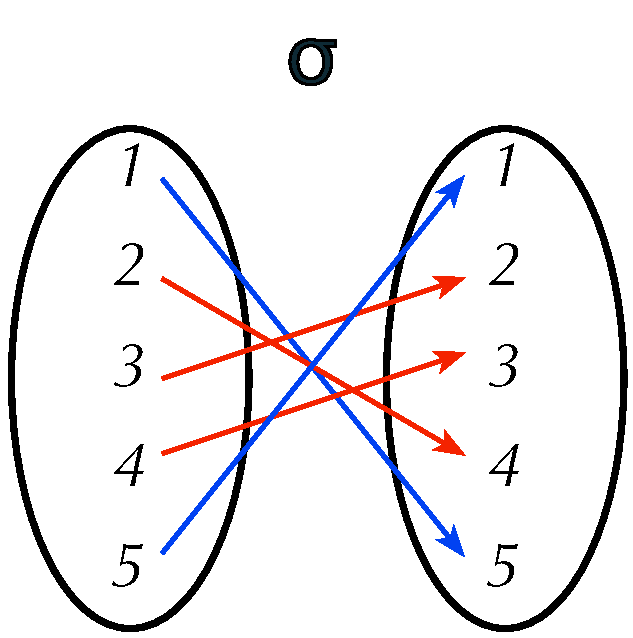
\includegraphics[height=30mm]{pics/cycledecomp.pdf}
	\begin{block}{Beispiel}
	\begin{itemize}
	\item f\ue r $n=5$ betrachte die Permutation
		\begin{align*}
			\sigma:1&\mapsto5&2&\mapsto4&3&\mapsto2&4&\mapsto3&5&\mapsto1
		\end{align*}
	\item die Zykeldarstellung lautet
		\begin{align*}
			\sigma&=(1\quad 5)\circ(2\quad 4\quad 3).
		\end{align*}
	\end{itemize}
	\end{block}
\end{frame}

\begin{frame}\frametitle{Zusammenfassung}
\begin{itemize}
\item Die symmetrische Gruppe besteht aus allen Permutationen von $n$ Elementen.
\item Gruppenoperation ist die Konkatenation von Abbildungen $\circ$.
\item Das Signum ist ein Beispiel f\ue r einen Homomorphismus.
\item Zerlegung von Permutationen in Zykel
\end{itemize}
\end{frame}

\end{document}
